\subsection{Spheroidal fluid particles}

Many studies have been conducted to determine the influence of the droplets' deformation on suspension Rheology \citet{goddard1967nonlinear,lhuillier1987phenomenology,maffettone1998equation}.
Most of the authors considered the Rheology of such an emulsion for neutrally buoyant droplets in linear flows. 
In this work, we would like to present a more general, but non-closed yet framework. 
As a first step to describe the rheology we are interested in the kinematics   and dynamic of a single deformable drop. 
At this stage the only restriction that we make about the drop is that it possesses oblate spheroidal shape. 
This is consistent with shape that adopt buoyant droplets or bubbles in fluid. 

\subsubsection*{Shape of the droplet}
We consider oblate spheroidal droplets as it is depicted \ref{fig:scheme_spheroid}. 
\begin{figure}[h!]
    \centering
    \hfill
    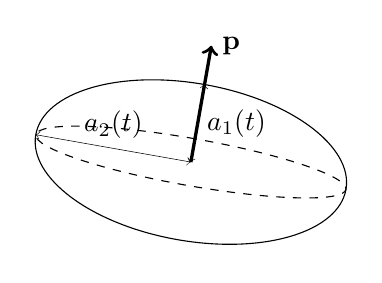
\begin{tikzpicture}[rotate=80]
        \draw(0,0) ellipse (1 cm and 2 cm);
        \draw[dashed](0,0) ellipse (0.3 cm and 2 cm);
        \draw[<->,very thin](0,0) --++ (1,0)node[midway,right]{$a_1(t)$};
        \draw[->,very thick](0,0) --++ (1.5,0)node[right]{$\textbf{p}$};
        \draw[<->,very thin](0,0) --++ (0,2)node[midway,above]{$a_2(t)$};
    \end{tikzpicture}
    \hfill
    \caption{Scheme of an  oblate spheroid oriented along the unit vector \textbf{p} with $a_1(t)$ and $a_2(t)$ the length of the semi axes of the spheroid.
    Note that when the drop is spherical we have $a_1=a_2=a$}
    \label{fig:scheme_spheroid}
\end{figure}
This shape might be described completely by the conformation tensor, $\textbf{C}_\alpha$.
This tensor is defined such that its eigenvalues are the dimensionless square semi axis length minus one, that is,
\begin{equation*}
    \textbf{C}_\alpha
    =  C_1\textbf{pp}
    + C_2 (\textbf{I} - \textbf{pp}),
\end{equation*}
where $C_i = \left(\frac{a_i}{a}\right)^2 - 1$. 
By a straightforward integral computation one can show that the second moment of mass is linked to the conformation tensor through the expression : $\textbf{M}_\alpha = \frac{m_\alpha a^2}{5}(\textbf{C}_\alpha + \textbf{I})$. 
Additionally, note that due to the volume conservation we have : $ a_2^2 = a^3 /a_1$. 
In terms of eigenvalues this gives : $(C_1+1) = (C_2+1)^{-2}$, 
Note that if we consider small deformations $C_1 = [(C_2+1)^{-2} - 1]= -2 C_2 + \mathcal{O}(C_2^2)$. 
Consequently, for small deformation $\textbf{I}:\textbf{C}_\alpha = C_1 + 2C_2 = 0$. 
Anyhow, the ellipsoid shape is completely determined by one scalar value $C_1$ or $C_2$ and the orientation tensor $\textbf{p}$ such that, 
\begin{equation*}
    \textbf{C}_\alpha
    =  -2 C_2\textbf{pp} 
    + C_2 (\textbf{I} - \textbf{pp}). 
\end{equation*}
Additionally, the point on the droplet's surface must respect $\FF_\alpha(\textbf{x},t) = 0$ where $\FF_\alpha$ is the distance function of the particle and is defined as, 
\begin{equation*}
    \FF_\alpha(\textbf{x},t) = \textbf{rr}:(\textbf{C}_\alpha + \textbf{I}) -a^2.  
    \label{eq:distance_function}
\end{equation*}


\subsubsection*{The droplet's internal velocity}


We know that an isolated droplet in creeping flow with translating motion exhibit internal motion known as Hill vortexes, see \ref{fig:flowlines} (b). 
For a drop immersed in an unbounded linear flow, still in stokes flows, we can derive an analytical solution such that $\textbf{w}_2^0 \sim \textbf{rrr}$, see \ref{fig:flowlines} (a). 
If slightly more inertial effects are present one might find that the internal motion are close to hill's vortexes but with an overall oblate spheroidal shape, see \ref{fig:flowlines} (c). 
In these cases the droplet's internal velocity fields is a steady solution.
Nevertheless, for a droplet to go from case (b) to case (c) a deformation must occur. 

To account for this deformation in our case we assume that the secondary velocity field that is responsible for the deformation is purely a linear function of the position. 
The internal velocity field of a particle under homogeneous linear deformation can be described as such, $\textbf{w}_2^0 = \bm\Gamma_\alpha \cdot \textbf{r}$. 
We have introduced, $\bm\Gamma_\alpha$, the mean velocity gradient inside the particle, which symmetric part : $\textbf{E}_\alpha$, represents the rate of strain, and skew symmetric part : $\bm\Omega_\alpha$, represents the angular velocity. 

\begin{figure*}
    \centering
    \begin{tikzpicture}
        \node (img3) at (0.6\textwidth,0) {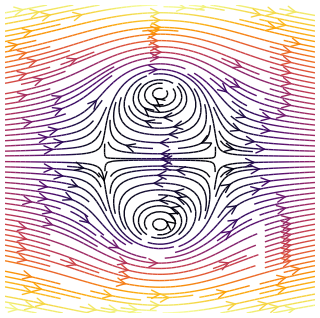
\includegraphics[width=0.3\textwidth,angle=270]{image/Rising_def_Stokes.png}};
        \node (img2) at (0.3\textwidth,0) {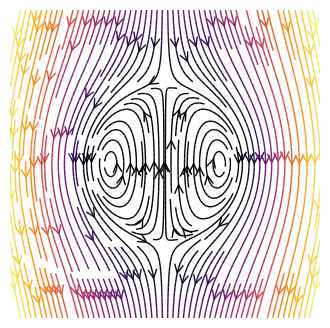
\includegraphics[width=0.3\textwidth]{image/Rising_Stokes.png}};
        % \draw (0.45\textwidth,0)node{$\rightarrow$};
        % \draw (0.45\textwidth,0.4cm)node{$\bm\Gamma_\alpha\cdot \textbf{r}$};
        \node (img1) at (0.0\textwidth,0) {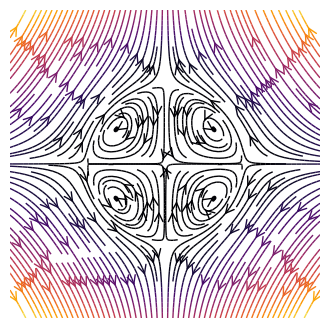
\includegraphics[width=0.3\textwidth]{image/Shear_Stokes.png}};
        \draw (img3.south)node{(c)};
        \draw (img2.south)node{(b)};
        \draw (img1.south)node{(a)};
    \end{tikzpicture}
    \caption{Three examples of steady state flow lines plots of an isolated droplet immersed into a viscous fluid. 
    (a) Rising sphere in uniform stokes flow (analytical solution in \ref{ap:Translating_sphere}). 
    (b) Fixed droplet in extensional flow (analytical solution in \ref{ap:Translating_sphere}).
    (c) Deformed droplet in rising motion (analytical solution of \citet{taylor1964deformation}). }
    \label{fig:flowlines}
\end{figure*}
To summarize, we assume that the inner velocity field of the drop can be decomposed into two distinct part. 
The first one is the steady state component, examples are : hill's vortex for spherical and oblate spheroidal drop in steady linear motion, the inner velocity field of a drop in steady linear flows, and so on. 
The second contribution is the inner velocity fields that alter the drop's shape, this field is assumed linear with the position and homogeneous, that is $\bm\Gamma\cdot \textbf{r}$. 
Adopting these definitions, the particle internal velocity is written, 
\begin{equation}
    \textbf{w}_{2,i}^0(\textbf{x}_\alpha)
    = \bm\Gamma_{\alpha,ik}(t) \cdot \textbf{r}_k
    + \textbf{w}^{s}_{2,i}(t,\textbf{r})
    =\bm{\Omega}_{\alpha,ik}\cdot \textbf{r}_k
    + \textbf{E}_{\alpha,ik} \cdot \textbf{r}_k
    + \textbf{w}^{s}_{2,i}(t,\textbf{r})
    \label{eq:def_vel}
\end{equation}
Where we introduced the vector $\textbf{w}^{s}_2(t,\textbf{r}) =\textbf{w}^{0}_{2,i}(t,\textbf{r})  - \bm\Gamma_{\alpha,ik}(t) \cdot \textbf{r}_k$ which represents all the internal motions that does not alter the drop's shape. 

An important consequence of this definition is that the integral on the RHS of \ref{eq:dt_S_alpha} is null when $\textbf{w}_{2,i}^0 = \textbf{w}_{2,i}^s$. 
This can be shown by re writting the second moment of mass equation with the use of the velocity decomposition.
This yields,
\begin{equation*}
    \ddt \textbf{M}_{\alpha,ik}
    = 
    \textbf{M}_{\alpha,ik} \cdot \bm\Gamma_{\alpha,kj}
    +  \bm\Gamma_{\alpha,ki} \cdot \textbf{M}_{\alpha,jk}
    +
    \intO{ 
        \textbf{w}_{2,i}^s\textbf{r}_j
        + \textbf{r}_i\textbf{w}_{2,j}^s
    }
\end{equation*}
In the cases where $\bm\Gamma = 0$, the droplet shape remains steady, in this case $\ddt \textbf{M}_\alpha = 0$ and $\intO{\textbf{w}^{s}_{2,i} \textbf{r}_j + \textbf{r}_i \textbf{w}_{2,i}^s} = 0$. 
In the case where $\bm\Gamma \neq 0$ the droplets deform according to the linear velocity fields $\bm\Gamma\cdot \textbf{r}$.
Since we assumed that no other source of deformation are present than the latter, we must have $\intO{\textbf{w}^{s}_{2,i} \textbf{r}_j + \textbf{r}_i \textbf{w}_{2,i}^s} = 0$ so that $\textbf{w}^{s}_{2,i} $ doesn't contribute to the deformation nor the rotation.
This, means that $\textbf{w}^{s}_{2,i}$ is a velocity fields determined in  part by the instantaneous shape of the droplet and its , that does not alter the shape of the drop. 
Additionally, the angular momentum is assumed to be entirely described by $\textbf{M}_\alpha \cdot \bm\Omega_\alpha$ meaning that, $\textbf{r} \textbf{w}_{2}^s$ plays no role at all in the total particle's moment of momentum.
This kind of fields is encountered in linear skew symmetric flows where the rotation is homogeneous and follow the carrier fluid vorticity. 
Anyhow, this velocity decomposition has the plaisent property that $\intO{\textbf{w}^{s}_{2,i} \textbf{r}_j} = 0$ at all time, which will simplify the equaitons of motions. 

Now some constrain should apply on the tensor $\textbf{E}_\alpha$.
Indeed, the mass conservation inside the particle \ref{eq:dt_rho} impose $\div \textbf{u}_2^0 = \textbf{E}_\alpha : \textbf{I}= 0$, where it is assumed that $\div \textbf{w}_2^s =0$. 
Also, note that to preserve the spheroidal shape of the particle we must assume that the particle's rate of strain principal direction is the same as the droplet's shape principal axis. 
In other worlds, $\textbf{E}_\alpha$ must have the same eigenbasis as $\textbf{C}_\alpha$. 
Making up with these two constrain leads to the expression : $\textbf{E}_\alpha = -2 E_2 \textbf{pp} + E_2 (\textbf{I}- \textbf{pp})$, where $E_2$ is the second eigenvalue of $\textbf{E}_\alpha$. 


As it is demonstrated in \ref{ap:Translating_sphere} the internal motion of an isolated spherical drop, such as the one in \ref{eq:def_vel}, is entirely determined  from $\textbf{u}_1$,$\grad\textbf{u}_1$,$\textbf{u}_\alpha$ and so on. 
Therefore, it is reasonable to think that in a more general case, $\textbf{w}_2^s$ might be entirely determined by the carrier fluid and particles' properties, namely, $\textbf{u}_\alpha$ $\textbf{C}_\alpha$, $\textbf{u}_1$ $\grad\textbf{u}_1$ and for non-dilute flows we might have $\phi_2$ or more complicated functions. 
Thus, from now on we consider that the internal velocity $\textbf{w}^{s}_2(t,\textbf{r})$ is not part of the particle' unknown, but rather is a closure term. 
Consequently, in this problem a single droplet is described exhaustively by, $\textbf{x}_\alpha, \textbf{u}_\alpha, \textbf{C}_\alpha$ and $\bm\Gamma_\alpha$. 
This requires two additional equations one for $\textbf{C}_\alpha$ and another for $\bm\Gamma_\alpha$. 

\subsubsection*{Evolution equations}

Before diving into the complexities of the second moment of mass and first moment of momentum equations, we must reformulate the integrals appearing in the former equation in terms of $\textbf{C}_\alpha$ and $\bm\Gamma_\alpha$.  
According to the preceding remarks the integrals appearing in \ref{eq:dt_M_alpha} and \ref{eq:dt_P_alpha} can be reformulated according to, 
\begin{align}
    \intO{(\textbf{rw}_2^0 )_{ij}+ (\textbf{w}_2^0 \textbf{r})_{ij}} 
    =\frac{m_\alpha a^2}{5}\left[
        \textbf{C}_{\alpha,ik} \cdot \bm\Gamma_{\alpha,jk}
        +  \bm\Gamma_{\alpha,ik} \cdot \textbf{C}_{\alpha,jk}
        +  \bm\Gamma_{\alpha,ij} + \bm\Gamma_{\alpha,ij}
    \right] 
    \\
    \intO{\rho_2 \textbf{w}_{2,i}^0\textbf{w}_{2,j}^0}
    =\frac{m_\alpha a^2}{5} \left[
        \bm\Gamma_{\alpha,jl}\bm\Gamma_{\alpha,ik} \textbf{C}_{\alpha,kl} 
            + \bm\Gamma_{\alpha,jk}\bm\Gamma_{\alpha,ik} 
    \right]  
        +\intO{\rho_2 \textbf{w}_{2,i}^s\textbf{w}_{2,j}^s}
    \\
    \label{eq:sigma_2_def}
    \intO{\bm\sigma_{2,ij}^0}
    =
    \mu_2 v_\alpha [\bm\Gamma_{\alpha,ij} + \bm\Gamma_{\alpha,ij}]
    - \intO{p_2^0} \textbf{I}_{ij}
    + \mu_2 \intS{(\textbf{n}_i \textbf{w}_{2,j}^s + \textbf{n}_j \textbf{w}_{2,i}^s)}
    \\
    \label{eq:sigma_I_def}
    \intS{\bm\sigma_{I,ij}^0}
    = \frac{2 \gamma v_\alpha }{a} \textbf{I}_{ij} - \frac{4 \gamma v_\alpha }{5 a} \textbf{C}_{\alpha,ij}
    +\mathcal(|\textbf{C}|^2)
\end{align}
These expressions are direct consequences of the velocity decomposition.
The surface tension integral has been computed based on \ref{eq:distance_function}.
Indeed, using the distance function, one can derive an expression for the surface normal, that is, $\textbf{n} = \frac{\grad \FF}{(\grad \FF\cdot\grad \FF)^{1/2}}$, and the local curvature $\div \textbf{n}$, in terms of $\textbf{C}_\alpha$\citep{nadim1996concise}.
Then, since $\bm\sigma_{I,ij}^0 = \gamma (\textbf{I}- \textbf{nn})$ one is able to compute the surface integral \ref{eq:sigma_I_def} and obtain an exact, or trucated solution. 
Here we give the results in the limit of small $C = |\textbf{C}_\alpha|$ at the first order. 
Indeed, in any case the spheroidal shape remains valid under small deformation assumption, therefor no need to consider the higher order terms. 

Injecting these expressions into \ref{eq:dt_M_alpha} and \ref{eq:dt_P_alpha} gives directly, 
\begin{align}
    \label{eq:dt_C_alpha}
    &\ddt \textbf{C}_{\alpha,ij}
    = \textbf{C}_{\alpha,ik} \cdot \bm\Gamma_{\alpha,jk}
    +  \bm\Gamma_{\alpha,ik} \cdot \textbf{C}_{\alpha,jk}
    +  \bm\Gamma_{\alpha,ij} + \bm\Gamma_{\alpha,ij}
    ,\\
    &\frac{a^2  m_\alpha}{5} \ddt( 
        \textbf{C}_{\alpha,ik} \cdot \bm\Gamma_{\alpha,jk}
        -  \bm\Gamma_{\alpha,ik} \cdot \textbf{C}_{\alpha,jk}
        +  
        \bm\Gamma_{\alpha,ij} - \bm\Gamma_{\alpha,ij}
    )
    =  
    \intS{(\textbf{r}\bm\sigma_2^0- \bm\sigma_2^0\textbf{r})\cdot \textbf{n}}\\
    &\frac{m_\alpha a^2}{10}\ddt^2 \textbf{C}_{\alpha,ij}
    - \frac{m_\alpha a^2}{5}[
        \bm\Gamma_{\alpha,jl}\bm\Gamma_{\alpha,ik} \textbf{C}_{\alpha,kl} 
        + \bm\Gamma_{\alpha,jk}\bm\Gamma_{\alpha,ik} 
    ]
    + \mu_2 v_\alpha (\bm \Gamma_{p,ij}+\bm \Gamma_{p,ji})
    - \frac{ \gamma v_\alpha }{ a} \left(\frac{4}{5}
        \textbf{C}_{\alpha,ij}
        -2 \textbf{I}_{ij}
    \right)\nonumber\\
    &= \frac{1}{2}\intS{(\textbf{r}\bm\sigma_2^0+ \bm\sigma_2^0\textbf{r})\cdot \textbf{n}}
    + \intO{p_2^0 \textbf{I}_{ij}}
    - \intS{\mu_2 (\textbf{n}_i \textbf{w}_{2,j}^s + \textbf{n}_j \textbf{w}_{2,i}^s)}
    - \intO{\rho_2 \textbf{w}_{2,i}^s\textbf{w}_{2,j}^s} \\
    &- \frac{m_\alpha a^2}{5}[
        \bm\Gamma_{\alpha,il}\bm\Gamma_{\alpha,ik} \textbf{C}_{\alpha,kl} 
        + \bm\Gamma_{\alpha,ik}\bm\Gamma_{\alpha,ik} 
    ]
    + 3 \frac{ 2 \gamma v_\alpha }{ a} 
= \frac{1}{2}\intS{\textbf{r}\cdot \bm\sigma_2^0\cdot \textbf{n}}
    + 3 \intO{p_2^0 }
    - \intO{\rho_2 \textbf{w}_{2,i}^s\cdot\textbf{w}_{2,j}^s} 
\end{align}
At this point one might remark that the equation for $\textbf{C}_\alpha$ is in fact an equation for the orientation and also deformation. 
To dissociate these two contribution one must first note that regardless of the deformation we have $\ddt \textbf{p} = \bm\Omega_\alpha \cdot \textbf{p}$.
Which means that the dyadic $\textbf{pp}$ follows the kinematics   equation :
\begin{equation*}
    \ddt \textbf{pp}_{\alpha,ij}
    =  \textbf{pp}_{\alpha,ik} \cdot \bm\Omega_{\alpha,jk}
    +  \bm\Omega_{\alpha,ik} \cdot \textbf{pp}_{\alpha,jk}.
\end{equation*}
By taking the double contracted product of \ref{eq:dt_C_alpha} with $\textbf{pp}$ one get the evolution equation for $\textbf{C}$ along the axis $\textbf{p}$, that is, an equation for the first eigenvalue $C_1$.
It yields, 
\begin{equation*}
    \ddt (\textbf{C}_{\alpha,ij} \textbf{pp}_{\alpha,ij})
    - \textbf{C}_{\alpha,ij} \ddt \textbf{pp}_{\alpha,ij} 
    = \textbf{pp}_{\alpha,ij} \textbf{C}_{\alpha,ik} \cdot \bm\Gamma_{\alpha,jk}
    + \textbf{pp}_{\alpha,ij}  \bm\Gamma_{\alpha,ik} \cdot \textbf{C}_{\alpha,jk}
    + \textbf{pp}_{\alpha,ij}  \bm\Gamma_{\alpha,ij} + \bm\Gamma_{\alpha,ij}
\end{equation*}
This equation can be considerably simplified.
Firstly note that $\textbf{C}_{\alpha,ij} \textbf{p}_{\alpha,j} = C_1 \textbf{p}_{\alpha,i}$. 
Equally, $\textbf{E}_{\alpha,ij} \textbf{pp}_{\alpha,ij} =E_1$
Second, note that the double contracted product of any skew symmetric tensor, such as $\bm\Omega_{\alpha,ij}$ and a symmetric tensor, let say $\textbf{pp}_{\alpha,ij}$ is always zero, i.e. $\bm\Omega_{\alpha,ij}\textbf{pp}_{\alpha,ij} = 0$.
Making use of these two properties yields the simpler equation : 
\begin{equation*}
    \ddt C_1
    = 2E_1(C_1+1)
\end{equation*}
Or in other worlds we have the relations : $2 E_1 = \ddt \ln(C_1+1) = - 2 \ddt \ln(C_2+1) = - E_2 $. 
This just means that the derivative of the deformation is the rate of strain. 

The same can be done for the symmetric part of the moment of momentum equation, it gives, 
\begin{align*}
    \frac{m_\alpha a^2}{10}\ddt^2 \textbf{C}_1
    - \frac{m_\alpha a^2}{10}\ddt \textbf{C}_{\alpha,ij} \ddt \textbf{pp}_{\alpha,ij}
    - \frac{m_\alpha a^2}{5}[
        E_2^2(C_1 + 1)
        +
        \bm\Omega_{\alpha,jl}\bm\Omega_{\alpha,ik} (\textbf{C}_{\alpha,kl} + \textbf{I}_{ij})\textbf{pp}_{\alpha,ij}
    ] \\
    + \mu_2 v_\alpha 2E_1
    - \frac{ \gamma v_\alpha }{ a} \left(\frac{4}{5}
        C_1
        -2 
    \right)\nonumber\\
    = \frac{1}{2}\intS{(\textbf{r}\bm\sigma_2^0+ \bm\sigma_2^0\textbf{r})\cdot \textbf{n}}\textbf{pp}_{\alpha,ij}
    + \intO{p_2^0 }
    - \intS{\mu_2 (\textbf{n}_i \textbf{w}_{2,j}^s + \textbf{n}_j \textbf{w}_{2,i}^s)}\textbf{pp}_{\alpha,ij}
    - \intO{\rho_2 \textbf{w}_{2,i}^s\textbf{w}_{2,j}^s} \textbf{pp}_{\alpha,ij}
\end{align*}
As these terms are rather tricky it is worth noting that we have used,  
\begin{align*}
    \ddt \textbf{C}_{\alpha,ij} \ddt \textbf{pp}_{\alpha,ij}
    = (\textbf{C}_{\alpha,ik} \cdot \bm\Gamma_{\alpha,jk}
    +  \bm\Gamma_{\alpha,ik} \cdot \textbf{C}_{\alpha,jk}
    +  2\textbf{E}_{\alpha,ij} )
    (\textbf{pp}_{\alpha,ik} \cdot \bm\Omega_{\alpha,jk}
    +  \bm\Omega_{\alpha,ik} \cdot \textbf{pp}_{\alpha,jk})\\
    =
    2 C_1 \textbf{pp}_{\alpha,kl}\Omega_{\alpha,jk}\Omega_{\alpha,jl}
    + 2 \textbf{C}_{\alpha,ik} \textbf{pp}_{\alpha,jl}
    \Omega_{\alpha,jk}\Omega_{\alpha,il}\\
    [ \bm\Gamma_{\alpha,il}\bm\Gamma_{\alpha,ik} \textbf{C}_{\alpha,kl} 
        + \bm\Gamma_{\alpha,ik}\bm\Gamma_{\alpha,ik} ]
    \textbf{pp}_{\alpha,ij}
    =
    E_1^2(1+C_2) + (\textbf{C}_{\alpha,kl} + \textbf{I}_{ij})  \textbf{pp}_{\alpha,ij} \bm\Omega_{\alpha,jl}\bm\Omega_{\alpha,ik}
\end{align*}
Since these are dummy indices note that by permuting $k\to i$ and $l\to k$ we could have, 
\begin{align*}
    (\textbf{C}_{\alpha,kl} + \textbf{I}_{kl})  \textbf{pp}_{\alpha,ij} \bm\Omega_{\alpha,jl}\bm\Omega_{\alpha,ik}
    = 
    (\textbf{C}_{\alpha,ik} + \textbf{I}_{ik})  
    \textbf{pp}_{\alpha,jl} 
    \bm\Omega_{\alpha,jk}
    \bm\Omega_{\alpha,li}\\
    = 
    \textbf{C}_{\alpha,ik} 
    \textbf{pp}_{\alpha,jl} 
    \bm\Omega_{\alpha,jk}
    \bm\Omega_{\alpha,li}
    + 
    \textbf{pp}_{\alpha,kl} \bm\Omega_{\alpha,jk} \bm\Omega_{\alpha,jl}
    \\
\end{align*}
which is exactly the same as the previous expression except for first terms which is minus the previous expression. 
Ultimately, we obtain, 
\begin{align*}
    - \frac{m_\alpha a^2}{10}
    (2 C_1 \textbf{pp}_{\alpha,kl}\Omega_{\alpha,jk}\Omega_{\alpha,jl}
    - 2 \textbf{C}_{\alpha,ik} \textbf{pp}_{\alpha,jl}
    \Omega_{\alpha,jk}\Omega_{\alpha,li})
    - \frac{m_\alpha a^2}{5}
    (
        \textbf{C}_{\alpha,ik} 
    \textbf{pp}_{\alpha,jl} 
    \bm\Omega_{\alpha,jk}
    \bm\Omega_{\alpha,li}
    + 
    \textbf{pp}_{\alpha,kl} \bm\Omega_{\alpha,jk} \bm\Omega_{\alpha,jl}
    )
    = \\
    - \frac{m_\alpha a^2}{5}
    (C_1 \textbf{pp}_{\alpha,kl}\Omega_{\alpha,jk}\Omega_{\alpha,jl}
)
    - \frac{m_\alpha a^2}{5}
    ( 
    \textbf{pp}_{\alpha,kl} \bm\Omega_{\alpha,jk} \bm\Omega_{\alpha,jl}
    )
    = 
    - \frac{m_\alpha a^2}{5}
     \textbf{pp}_{\alpha,kl}\Omega_{\alpha,jk}\Omega_{\alpha,jl} (C_1 +1 )
\end{align*}
That is as far as we can go for the skew part equation. 

Now regarding the trace only the terms on the LHS appear, 
\begin{equation*}
    \bm\Gamma_{\alpha,il}\bm\Gamma_{\alpha,ik} \textbf{C}_{\alpha,kl} 
        + \bm\Gamma_{\alpha,ik}\bm\Gamma_{\alpha,ik} 
        = 
        E_1^2 (C_1 +1)
        + 2E_2^2 (C_2+1)
        + \bm\Omega_{\alpha,il}
        \bm\Omega_{\alpha,ik}(
            \textbf{C}_{\alpha,kl}
            + \textbf{I}_{\alpha,kl}
        )
\end{equation*}
The trace equation reads, 
\begin{align*}
    \frac{m_\alpha a^2}{10}\ddt(C_1+2C_2)
    - \frac{m_\alpha a^2}{5}        
    [E_1^2 (C_1 +1)
    + 2E_2^2 (C_2+1)
    + \bm\Omega_{\alpha,il}
    \bm\Omega_{\alpha,ik}(
        \textbf{C}_{\alpha,kl}
        + \textbf{I}_{\alpha,kl}
    )]
    +  \frac{  \gamma v_\alpha }{ a} 
    [\frac{4}{5}(C_1+2C_2) + 6]\\
    =\frac{1}{2} \intS{\textbf{r}\cdot \bm\sigma_2^0\cdot \textbf{n}}
    + 3 \intO{p_2^0 }
    - \intO{\rho_2 \textbf{w}_{2,i}^s\cdot\textbf{w}_{2,j}^s} 
\end{align*}
In the end the symmetric part equation reads, 
\begin{align*}
    \frac{m_\alpha a^2}{10}\ddt^2 C_1
    - (C_1 + 1) \frac{m_\alpha a^2}{5}(
         E_1^2
        + \textbf{pp}_{\alpha,kl}\bm\Omega_{\alpha,jk}\bm\Omega_{\alpha,jl})
    + \mu_2 v_\alpha 2 E_1
    - \frac{ \gamma v_\alpha }{ a} \left(\frac{4}{5}
        C_1
        -2 
    \right)\nonumber\\
    = \frac{1}{2}\intS{(\textbf{r}\bm\sigma_2^0+ \bm\sigma_2^0\textbf{r})\cdot \textbf{n}}\textbf{pp}_{\alpha,ij}
    + \intO{p_2^0 }
    - \intS{\mu_2 (\textbf{n}_i \textbf{w}_{2,j}^s + \textbf{n}_j \textbf{w}_{2,i}^s)}\textbf{pp}_{\alpha,ij}
    - \intO{\rho_2 \textbf{w}_{2,i}^s\textbf{w}_{2,j}^s} \textbf{pp}_{\alpha,ij}
\end{align*}

Subtracting the trace expression to the latter expression latter gives, 
\begin{align*}
    \frac{m_\alpha a^2}{10}\ddt^2 (-2C_2)
    - (C_1 + 1) \frac{m_\alpha a^2}{5}(
         E_1^2
        + \textbf{pp}_{\alpha,kl}\bm\Omega_{\alpha,jk}\bm\Omega_{\alpha,jl})
    + \mu_2 v_\alpha 2 E_1
    - \frac{ \gamma v_\alpha }{ a} \left(\frac{4}{5}
        C_1
        -2 
    \right)\nonumber\\
    = \frac{1}{2}\intS{(\textbf{r}\bm\sigma_2^0+ \bm\sigma_2^0\textbf{r}- \bm\sigma_2^0\cdot \textbf{r})\cdot \textbf{n}}\textbf{pp}_{\alpha,ij}
    - \intS{\mu_2 (\textbf{n}_i \textbf{w}_{2,j}^s + \textbf{n}_j \textbf{w}_{2,i}^s)}\textbf{pp}_{\alpha,ij}\\
    - \intO{\rho_2 \textbf{w}_{2,i}^s\textbf{w}_{2,j}^s-\rho_2 \textbf{w}_{2,i}^s\cdot\textbf{w}_{2,j}^s} \textbf{pp}_{\alpha,ij}
\end{align*}



We now are seeking to an asymptotic solution. 


\tb{
    \begin{itemize}
        \item Remove the factor $m a^2$ or do something for clearty
        \item Try to introduce the dimensionless shit 
        \item Maybe remove the trace before deriving this whole equations, actually juste need to check if  
    \end{itemize}
}

\section*{Re-derivation but more easy}
All these went way to complicated. 
So here is a more consize derivation that does keep track of the physics. 
We describe the geometry of the particle with the second moment of mass tensor, 
\begin{equation*}
    \textbf{M}_{\alpha,ij} 
    =\frac{m_\alpha a^2}{5} \textbf{M}_{\alpha,ij}^*
    = \frac{m_\alpha a^2}{5}\left[
        \left(
            \frac{a_1}{a}
        \right)^2\textbf{pp}
        + 
        \left(
            \frac{a_1}{a}
        \right)^2(\textbf{I}- \textbf{pp})
    \right]
    = 
\end{equation*}
This tensor has several notable properties, the volume conservation : $a_1 a_2^2 = a^3$ which means that $\textbf{M}_\alpha^*$ has two eigenvalues linked through $M_1 = M_2^{-2}$. 
By considering small deformation $(a_2/a) - 1= \varepsilon$ we can state that $M_1 = M_2^{-2} = 1 - 2 (M_2 - 1 ) + \mathcal{O}((M_2-1)^2)$. 
Alternatively, if $M_1 = M_1^(0) + \varepsilon M_2^(1) + \ldots$. 


Let's now remformulate the integral of the problem namely, 
\begin{align}
    \intO{(\textbf{rw}_2^0 )_{ij}+ (\textbf{w}_2^0 \textbf{r})_{ij}} 
    = \textbf{M}_{\alpha,ik} \cdot \bm\Gamma_{\alpha,jk}
        +  \bm\Gamma_{\alpha,ik} \cdot \textbf{M}_{\alpha,jk}
    \\
    \intO{\rho_2 \textbf{w}_{2,i}^0\textbf{w}_{2,j}^0}
    = \bm\Gamma_{\alpha,jl}\bm\Gamma_{\alpha,ik} \textbf{M}_{\alpha,kl}  
        +\intO{\rho_2 \textbf{w}_{2,i}^s\textbf{w}_{2,j}^s}
    \\
    \intO{\bm\sigma_{2,ij}^0}
    =
    2 \mu_2 v_\alpha \textbf{E}_{\alpha,ij}
    - \intO{p_2^0} \textbf{I}_{ij}
    + \mu_2 \intS{(\textbf{n}_i \textbf{w}_{2,j}^s + \textbf{n}_j \textbf{w}_{2,i}^s)}
    \\
    \intS{\bm\sigma_{I,ij}^0}
    = \frac{\gamma v_\alpha }{a} \left[
        2\textbf{I}_{ij} 
        - \frac{4 \gamma v_\alpha }{5 a} (\textbf{M}_{\alpha,ij}^* - \textbf{I}_{\alpha,ij})
    \right]
    +\mathcal(O)(\textbf{C}\cdot \textbf{C})\\
    s_\alpha 
    = 4\pi a^2 (1+\frac{\textbf{C}:\textbf{C}}{15})
\end{align}
for the surface tension term is made of two terms, one corresponding to Laplace pressure and the other to the deviatoric stress. 

The equation for the orientation, second moment of mass torque, symmetric moment of momentum and trace of the moment of momentum reads, 
\begin{align*}
    \ddt \textbf{pp}_{\alpha,ij}
    = \textbf{pp}_{\alpha,ik} \cdot \bm\Omega_{\alpha,jk}
    +  \bm\Omega_{\alpha,ik} \cdot \textbf{pp}_{\alpha,jk}\\
    \ddt \textbf{M}_{\alpha,ij}
    = \textbf{M}_{\alpha,ik} \cdot \bm\Gamma_{\alpha,jk}
    +  \bm\Gamma_{\alpha,ik} \cdot \textbf{M}_{\alpha,jk}\\
    \ddt (\textbf{I}_{\alpha,ik}\bm\omega_{\alpha,k} )
    = 
    \intS{(\textbf{r}\times\bm\sigma_1^0\cdot \textbf{n})_i} \\
    \frac{1}{2}\ddt^2 \textbf{M}_{\alpha,ij}
    -  \bm\Gamma_{\alpha,jl}\bm\Gamma_{\alpha,ik} \textbf{M}_{\alpha,kl}  
    + 2 \mu_2 v_\alpha \textbf{E}_{\alpha,ij}
    + \frac{\gamma v_\alpha }{a} \left[
    2\textbf{I}_{ij} 
    - \frac{4 \gamma v_\alpha }{5 a} (\textbf{M}_{\alpha,ij}^* - \textbf{I}_{\alpha,ij})
    \right]\\
    = 
    \frac{1}{2}\intS{(\textbf{r}\sigma_1^0 + \sigma_1^0\textbf{r})\cdot \textbf{n}} 
    + \intO{\rho_2 \textbf{w}_{2,i}^s\textbf{w}_{2,j}^s}
    + \intO{p_2^0} \textbf{I}_{ij}
    - \mu_2 \intS{(\textbf{n}_i \textbf{w}_{2,j}^s + \textbf{n}_j \textbf{w}_{2,i}^s)}\\
    \frac{1}{2}\ddt^2 \textbf{M}_{\alpha,mm}
    -  \bm\Gamma_{\alpha,ml}\bm\Gamma_{\alpha,mk} \textbf{M}_{\alpha,kl}  
    + \frac{\gamma v_\alpha }{a} \left[
    2\textbf{I}_{mm} 
    - \frac{4 }{5 } (\textbf{M}_{\alpha,mm}^* - \textbf{I}_{\alpha,mm})
    \right]\\
    = 
    \intS{\textbf{r}_m\cdot\bm\sigma_{1,mk}^0\cdot \textbf{n}_k} 
    + \intO{\rho_2 \textbf{w}_{2,m}^s\cdot \textbf{w}_{2,m}^s}
    + \intO{p_2^0} \textbf{I}_{mm}
\end{align*}
What we are really interested in is the Deviatoric part of the stress equation, 
\begin{align*}
    \frac{1}{2}\ddt^2 (\textbf{M}_{\alpha,ij} - \frac{1}{3}\textbf{M}_{\alpha,mm} \textbf{I}_{ij})
    -   \textbf{M}_{\alpha,kl} 
    (\bm\Gamma_{\alpha,jl}\bm\Gamma_{\alpha,ik}  
    - \frac{1}{3}
    \bm\Gamma_{\alpha,ml}\bm\Gamma_{\alpha,mk}  
    \textbf{I}_{ij}
    )\\
    + 2 \mu_2 v_\alpha \textbf{E}_{\alpha,ij}
    - \frac{\gamma v_\alpha }{a} \left[
    \frac{4  }{5} (\textbf{M}_{\alpha,ij}^* - \frac{1}{3} \textbf{M}_{\alpha,mm}\textbf{I}_{\alpha,ij})
    \right]\\
    = 
    \frac{1}{2}\intS{(\textbf{r}\bm\sigma_1^0 + \bm\sigma_1^0\textbf{r} - \frac{2}{3}\textbf{r}\cdot \bm\sigma_1^0 \textbf{I})\cdot \textbf{n}} 
    + \intO{\rho_2 (\textbf{w}_{2,i}^s\textbf{w}_{2,j}^s - \frac{1}{3}\textbf{w}_{2,m}^s\textbf{w}_{2,m}^s \textbf{I}_{ij}) }
    - \mu_2 \intS{(\textbf{n}_i \textbf{w}_{2,j}^s + \textbf{n}_j \textbf{w}_{2,i}^s)}\\
\end{align*}
Introducing $\textbf{D}_{\alpha,ij}$ as the deviatoric part of $\textbf{M}_{\alpha,ij}$ yields,
\begin{align*}
    \frac{1}{2}\ddt^2 \textbf{D}_{\alpha,ij}
    -   \textbf{M}_{\alpha,kl} 
    (\bm\Gamma_{\alpha,jl}\bm\Gamma_{\alpha,ik}  
    - \frac{1}{3}
    \bm\Gamma_{\alpha,ml}\bm\Gamma_{\alpha,mk}  
    \textbf{I}_{ij}
    )
    + 2 \mu_2 v_\alpha \textbf{E}_{\alpha,ij}
    - \frac{\gamma v_\alpha }{a} 
    \frac{4  }{5} \textbf{D}_{\alpha,ij}
    \\
    = 
    \frac{1}{2}\intS{(\textbf{r}\bm\sigma_1^0 + \bm\sigma_1^0\textbf{r} - \frac{2}{3}\textbf{r}\cdot \bm\sigma_1^0 \textbf{I})\cdot \textbf{n}} 
    + \intO{\rho_2 (\textbf{w}_{2,i}^s\textbf{w}_{2,j}^s - \frac{1}{3}\textbf{w}_{2,m}^s\textbf{w}_{2,m}^s \textbf{I}_{ij}) }
    - \mu_2 \intS{(\textbf{n}_i \textbf{w}_{2,j}^s + \textbf{n}_j \textbf{w}_{2,i}^s)}\\
\end{align*}
The second moment of mass equation are still in tensor form. 
Similarly, the symmetric and skew part of the moment of momentum equation are both expressed in the laboratory frame. 
These reads quite complicated.
\subsubsection*{Local basis equation}
We want to write the previous equations in the local basis of the particle in order to be able to distinguish the deformation and rate of strain components from the rotational effects. 
Let's $\textbf{p}^1_i$, $\textbf{p}^2_i$ and $\textbf{p}^3_i$, be $3$ eigenvector of the tensor $\textbf{M}_{\alpha,ij}$, (or $\textbf{E}_{\alpha,ij}$). 
By convention, we consider that $\textbf{p}^1_i = \textbf{p}_i$, so that $\textbf{p}^2_i$ and $\textbf{p}^3_i$ are two arbitrarily oriented vector normal to $\textbf{pp}$. 
Since our geometry is for aft symmetric $\textbf{p}^1_i$, $\textbf{p}^2_i$ and $\textbf{p}^3_i$ constitutes an orthonormal basis. 
The derivative of the $a^{th}$ eigenvector yields, 
\begin{align*}
    \ddt \textbf{p}_i^a = \bm\Omega_{\alpha,ik}\cdot\textbf{p}_k^a
\end{align*}
where the orientation matrix is related to the angular velocity vector by $\epsilon_{kil}\bm\omega_l = \bm\Omega_{ik}$. 
Multiplying the previous equation to $\textbf{p}_j^b$ makes, 
\begin{align*}
    \textbf{p}_j^b\ddt \textbf{p}_i^a 
    = \bm\Omega_{\alpha,ik}\cdot\textbf{p}_k^a\textbf{p}_j^b\\
\end{align*}
Adding to this equation is transposed by applying the permutation  $i,a \to j,b$ yields an equation for the dyadic $ \textbf{p}_i^a \textbf{p}_j^b$, namely, 
\begin{align*}
    \ddt (\textbf{p}_i^a \textbf{p}_j^b)
    = \bm\Omega_{\alpha,ik}\cdot\textbf{p}_k^a\textbf{p}_j^b
    + \bm\Omega_{\alpha,jk}\cdot\textbf{p}_k^b\textbf{p}_i^a\\
\end{align*}

Any matrix $\textbf{A}_{ij}$ can be expressed in the basis,$\{\textbf{p}^1_i$, $\textbf{p}^2_i$, $\textbf{p}^3_i\}$. 
Indeed, we can express any second order tensor $\textbf{A}$ such that, 
\begin{equation*}
    \textbf{A}_{ij} 
    = 
    \sum_{a,b=1}^{3} 
    A^{ab}
    \textbf{p}_i^a \textbf{p}_j^b
\end{equation*}
Here $A^{ab}$ are the components of $\textbf{A}_{ij}$ in the reference frame $\{\textbf{p}^1_i$, $\textbf{p}^2_i$, $\textbf{p}^3_i\}$. 
They are defined as such that $A^{ab} = \textbf{A}_{ij}\textbf{p}^a_i\textbf{p}^b_j$. 
Because indeed, we have, 
\begin{equation*}
    \textbf{A}_{ij} \textbf{p}^a_i\textbf{p}^b_j
    = 
    \sum_{c,d=1}^{3} 
    A^{cd}
    \delta^{ca}
    \delta^{bd}
    = 
    A^{ab}
\end{equation*}
without the summation convention we might have, 
\begin{equation}
    \textbf{A}_{ij} \textbf{p}^a_i\textbf{p}^b_j
    = 
    A^{cd} \textbf{p}^c_i\textbf{p}^d_j\textbf{p}^a_i\textbf{p}^b_j
    = 
    A^{cd} \delta^{ca}\delta^{db}
    = 
    A^{ab}
\end{equation}
In fact the cross term vanish for \textbf{M} but let ignore that for the moment. 

It is clear that for $\mathbf{M}_{\alpha,ij}$ and $\textbf{E}_{\alpha,ij}$ the local coordinates $M^{ab}$ and $E^{ab}$ will be non-zero for $a=b$ since it is an eigenbasis. 
Now let's proceed to the projection of the second moment of mass equation. 
It yields, 
\begin{align*}
    \ddt (M^{ab})
    - \textbf{M}_{\alpha,ij}(
    \bm\Omega_{\alpha,ik}\cdot\textbf{p}_k^a\textbf{p}_j^b
    + \bm\Omega_{\alpha,jk}\cdot\textbf{p}_k^b\textbf{p}_i^a
    )
    = \textbf{M}_{\alpha,ik} \cdot \bm\Gamma_{\alpha,jk}\textbf{p}_i^a \textbf{p}_j^b
    +  \bm\Gamma_{\alpha,ik} \cdot \textbf{M}_{\alpha,jk}\textbf{p}_i^a \textbf{p}_j^b
\end{align*}
To simplify this equation note that, 
\begin{equation*}
    \textbf{M}_{\alpha,ij}\textbf{p}_k^a\textbf{p}_j^b
    = (\sum_{c,d=1}^3 M^{cd} \textbf{p}_i^c \textbf{p}_j^d) \textbf{p}_k^a\textbf{p}_j^b
    = \sum_{c,d=1}^3 M^{cd} \textbf{p}_i^c  \textbf{p}_k^a \delta^{bd}
    = \sum_{c,d=1}^3 M^{cb} \textbf{p}_i^c  \textbf{p}_k^a 
\end{equation*}
where we have used $\textbf{p}_j^d \textbf{p}_j^b = \delta_{db}$ since they are all unit normal vectors. 
in matrix notation over $c,d$ it reads, 
\begin{equation*}
    \textbf{M}_{\alpha,ij}\textbf{p}_k^a\textbf{p}_j^b
    = \textbf{M}^{cd}_\alpha \textbf{p}_i^c \textbf{p}_j^d \textbf{p}_k^a\textbf{p}_j^b
    = \textbf{M}^{cd}_\alpha \textbf{p}_i^c \textbf{p}_k^a\delta^{db}
    = \textbf{M}^{cb}_\alpha \textbf{p}_i^c \textbf{p}_k^a
\end{equation*}
In this basis note that $\textbf{M}^{cb}_\alpha = 0$ for any $c\neq b$.
\begin{equation}
    \textbf{M}^{cb}_\alpha \textbf{p}_i^c \textbf{p}_k^a \bm\Omega_{\alpha,ik}
    = 
    \textbf{M}^{cb}_\alpha \textbf{p}_i^c \textbf{p}_k^a 
    \bm\Omega_{\alpha}^{de} \textbf{p}^d_i\textbf{p}^e_k
    = 
    \textbf{M}^{cb}_\alpha  
    \bm\Omega_{\alpha}^{de} 
    \delta^{cd}
    \delta^{ae}
    = 
    \textbf{M}^{cb}_\alpha  
    \bm\Omega_{\alpha}^{ca} 
\end{equation}
In the end we just projected our scalar product in a new eigenbasis. 
In this new basis $\bm\Omega_{\alpha}^{ca}$ is still skew symmetric thus, if $b=a$ 
this tensor vanish. 
Let's do the permutation, 
\begin{equation}
    \textbf{p}_k^b\textbf{p}_j^a 
    \textbf{M}_{\alpha,ij} 
    \bm\Omega_{\alpha,ik} 
    = 
    \textbf{p}_k^b\textbf{p}_j^a 
    \textbf{M}^{\alpha,cd} \textbf{p}_i^c\textbf{p}_j^d
    \bm\Omega^{\alpha,ef} \textbf{p}_i^e\textbf{p}_k^f 
    = 
    \textbf{M}^{ca}_\alpha
    \bm\Omega^{cb}_\alpha
\end{equation}
\begin{equation}
    \textbf{p}_k^b\textbf{p}_i^a 
    \textbf{M}_{\alpha,ij} 
    \bm\Omega_{\alpha,jk} 
    = 
    \textbf{p}_k^b\textbf{p}_i^a 
    \textbf{M}^{\alpha,cd} \textbf{p}_i^c\textbf{p}_j^d
    \bm\Omega^{\alpha,ef} \textbf{p}_j^e\textbf{p}_k^f 
    = 
    \textbf{M}^{ad}_\alpha
    \bm\Omega^{db}_\alpha
\end{equation}
Since $\textbf{M}^{ab}$ is still symmetric it is reasonable to simplify this term. 
Additionally we have,
\begin{equation}
    \textbf{M}_{\alpha,ik}  \bm\Gamma_{\alpha,jk}\textbf{p}_i^a \textbf{p}_j^b
    = 
    \textbf{p}_i^a \textbf{p}_j^b
    \textbf{M}_\alpha^{cd} \textbf{p}^c_i \textbf{p}^d_k 
    \bm\Gamma_\alpha^{ef} \textbf{p}_j^e \textbf{p}_k^f
    = \delta^{ca}\delta^{be}\delta^{df}
     \textbf{M}_\alpha^{cd}
    \bm\Gamma_\alpha^{ef}
    = 
     \textbf{M}_\alpha^{ad}
    \bm\Gamma_\alpha^{bd}
    = 
    \textbf{M}_\alpha^{ad}
   (\textbf{E}_\alpha^{bd} + \bm\Omega^{bd})
\end{equation}
Again it is a simple scalar product, and the rotational term vanish for $a=b$. 
Permuting $i$ and $j$ as it is the case in the equation gives, 
\begin{equation}
    \textbf{M}_{\alpha,jk}  \bm\Gamma_{\alpha,ik}\textbf{p}_i^a \textbf{p}_j^b
    = 
    \textbf{p}_i^a \textbf{p}_j^b
    \textbf{M}_\alpha^{cd} \textbf{p}^c_j \textbf{p}^d_k 
    \bm\Gamma_\alpha^{ef} \textbf{p}_i^e \textbf{p}_k^f
    = \delta^{ae}\delta^{bc}\delta^{df}
     \textbf{M}_\alpha^{cd}
    \bm\Gamma_\alpha^{ef}
    = 
     \textbf{M}_\alpha^{bd}
    \bm\Gamma_\alpha^{ad}
    = 
    \textbf{M}_\alpha^{bd}
   (\textbf{E}_\alpha^{ad} + \bm\Omega^{ad})
\end{equation}
Overall we still get the same indices really but with $a$ and $b$ permuted. 


Now that we understood how it works we may write, 
\begin{align*}
    \ddt (\textbf{M}^{ab}_\alpha)
    = 
    + \textbf{M}_{\alpha,ij}(
    \bm\Omega_{\alpha,ik}\cdot\textbf{p}_k^a\textbf{p}_j^b
    + \bm\Omega_{\alpha,jk}\cdot\textbf{p}_k^b\textbf{p}_i^a
    )
    \textbf{M}_{\alpha,ik} \cdot \bm\Gamma_{\alpha,jk}\textbf{p}_i^a \textbf{p}_j^b
    +  \bm\Gamma_{\alpha,ik} \cdot \textbf{M}_{\alpha,jk}\textbf{p}_i^a \textbf{p}_j^b
\end{align*}
As, 
\begin{align*}
    \ddt (\textbf{M}^{ab}_\alpha)
    = 
    \textbf{M}^{cb}_\alpha\bm\Omega^{ca}_\alpha
    + \textbf{M}^{ac}_\alpha\bm\Omega^{cb}_\alpha
    + \textbf{M}^{ac}_\alpha \bm\Gamma^{bc}_\alpha 
    +  \bm\Gamma^{ac}_\alpha \textbf{M}^{bc}_\alpha
\end{align*}
Taking in account the fact that $\textbf{M}^{bc}_\alpha$ and $\textbf{E}^{bc}_\alpha$ are symmetric, and that $\bm\Omega^{ac}$ is skew symmetric we have, 
\begin{align*}
    \ddt (\textbf{M}^{ab}_\alpha)
    = 
    \textbf{M}^{ac}_\alpha \textbf{E}^{bc}_\alpha 
    +  \textbf{E}^{ac}_\alpha \textbf{M}^{bc}_\alpha
\end{align*}
For now we did not even make the assumption of \textbf{M} and \textbf{E} being diagonal, just that the basis rotate with \textbf{M}.
Taking in account that \textbf{M} is diagonal wa can re-write this expression by Introducing the unit vector $\textbf{I}_i = [1,1,1]$ such that $M_\alpha^a = \textbf{M}^{ab} \textbf{I}^b$ and same for \textbf{E} which eventually gives, 
\begin{align*}
    \ddt (M^i)
    = 
    2M^iE^i
\end{align*}
Or, 
\begin{align*}
    E^i = \ddt \ln(M^i)
\end{align*}

Now let's project the stresslet eq
\begin{align*}
    \frac{1}{2}\ddt^2 D^{ab}_\alpha
    - \frac{1}{2}\ddt (\textbf{p}_i^a\textbf{p}_j^b)
    -   \textbf{M}_{\alpha,kl} 
    (\bm\Gamma_{\alpha,jl}\bm\Gamma_{\alpha,ik}  
    - \frac{1}{3}
    \bm\Gamma_{\alpha,ml}\bm\Gamma_{\alpha,mk}  
    \textbf{I}_{ij}
    )
    + 2 \mu_2 v_\alpha \textbf{E}_{\alpha,ij}
    - \frac{\gamma v_\alpha }{a} 
    \frac{4  }{5} \textbf{D}_{\alpha,ij}
    \\
    = 
    \frac{1}{2}\intS{(\textbf{r}\bm\sigma_1^0 + \bm\sigma_1^0\textbf{r} - \frac{2}{3}\textbf{r}\cdot \bm\sigma_1^0 \textbf{I})\cdot \textbf{n}} 
    + \intO{\rho_2 (\textbf{w}_{2,i}^s\textbf{w}_{2,j}^s - \frac{1}{3}\textbf{w}_{2,m}^s\textbf{w}_{2,m}^s \textbf{I}_{ij}) }
    - \mu_2 \intS{(\textbf{n}_i \textbf{w}_{2,j}^s + \textbf{n}_j \textbf{w}_{2,i}^s)}\\
\end{align*}

\subsubsection*{Projection on the principal axes}


Where the identity matrix is related to the inertia tensor through $\textbf{I} = \textbf{M} - \frac{1}{2}(\textbf{M}:\textbf{I})\textbf{I}$. 

As we see now we can proceed to some simplification. 
First note that the deformation and rate of strain of the particles are actually linked through the conservation of volume of the particles. 
Thus, in principle one scalar value for each is needed. 
The torque equation might be re-written in its local frame of reference to. 
To do so we recall that, 
\begin{equation*}
    \textbf{M}_{\alpha,ij} 
    = M_1 \textbf{pp}_{\alpha,ij}
    + M_2 (\textbf{I}_{ij} - \textbf{pp}_{\alpha,ij})
    \textbf{E}_{\alpha,ij} 
    = E_1 \textbf{pp}_{\alpha,ij}
    + E_2 (\textbf{I}_{ij} - \textbf{pp}_{\alpha,ij})
\end{equation*}
and that $\bm\Omega_{\alpha,ij}$ is skew symmetric. 
In the following derivation we make use of the following identities which are all consequence that $A_{ij}B_{ij} = 0$ if $A$ is skew symmetric and $B$ symmetric. 
Indeed, we have, 
\begin{align*}
    \ddt \textbf{M}_{\alpha,ij}
    \ddt \textbf{pp}_{\alpha,ij}
    = 
    (\textbf{M}_{\alpha,ik}  \bm\Gamma_{\alpha,jk}
    +  \bm\Gamma_{\alpha,ik}  \textbf{M}_{\alpha,jk})
    (\textbf{pp}_{\alpha,ik}  \bm\Omega_{\alpha,jk}
    +  \bm\Omega_{\alpha,ik}  \textbf{pp}_{\alpha,jk})\\
    = 
    M_1  \bm\Omega_{\alpha,jk}
    \textbf{pp}_{\alpha,kl}  \bm\Omega_{\alpha,jl}
    +  \bm\Omega_{\alpha,ik}  \textbf{M}_{\alpha,jk}
    \textbf{pp}_{\alpha,il}  \bm\Omega_{\alpha,jl} \\
    + \textbf{M}_{\alpha,ik}  \bm\Omega_{\alpha,jk}
    \bm\Omega_{\alpha,il}  \textbf{pp}_{\alpha,jl}
    + M_1  \bm\Omega_{\alpha,ik}  
    \bm\Omega_{\alpha,il}  \textbf{pp}_{\alpha,kl}\\
    \frac{1}{2}\ddt \textbf{M}_{\alpha,ij}
    \ddt \textbf{pp}_{\alpha,ij}
    = 
     M_1  
     \bm\Omega_{\alpha,jk}
     \bm\Omega_{\alpha,jl}
    \textbf{pp}_{\alpha,kl}  
    +   
    \bm\Omega_{\alpha,jk}  
    \bm\Omega_{\alpha,il} 
    \textbf{M}_{\alpha,ik}
    \textbf{pp}_{\alpha,jl}  
\end{align*}
Equally we have, 
\begin{align*}
    \bm\Gamma_{\alpha,jl} \bm\Gamma_{\alpha,ik} \textbf{M}_{\alpha,kl} \textbf{pp}_{\alpha,ij}
    = 
    (\bm\Omega_{\alpha,jl}+\textbf{E}_{\alpha,jl}) (\bm\Omega_{\alpha,ik}+\textbf{E}_{\alpha,ik}) \textbf{M}_{\alpha,kl} \textbf{pp}_{\alpha,ij}\\
    = 
    \bm\Omega_{\alpha,jl}\bm\Omega_{\alpha,ik}\textbf{M}_{\alpha,kl} \textbf{pp}_{\alpha,ij}
    + \textbf{E}_{\alpha,jl} \textbf{E}_{\alpha,ik} \textbf{M}_{\alpha,kl} \textbf{pp}_{\alpha,ij}\\
    = 
    \bm\Omega_{\alpha,jl}
    \bm\Omega_{\alpha,ik}
    \textbf{M}_{\alpha,kl} 
    \textbf{pp}_{\alpha,ij}
    + E_1^2 M_1 \\
    = 
    - 
    \bm\Omega_{\alpha,jk}
    \bm\Omega_{\alpha,il}
    \textbf{M}_{\alpha,ik} 
    \textbf{pp}_{\alpha,jl}
    + E_1^2 M_1 \\
\end{align*}
Note that the first term is in fact the same as the second of the previous expression, they will cancel out. 

The terms appearing in the trace equation are,
\begin{align*}
    \bm\Gamma_{\alpha,il} \bm\Gamma_{\alpha,ik} \textbf{M}_{\alpha,kl}
    = 
    (\textbf{E}_{\alpha,il} + \bm\Omega_{\alpha,il}) 
    (\textbf{E}_{\alpha,ik} + \bm\Omega_{\alpha,ik})
    \textbf{M}_{\alpha,kl}\\
    = 
    \textbf{E}_{\alpha,il} 
    \textbf{E}_{\alpha,ik} 
    \textbf{M}_{\alpha,kl}
    + 
    \bm\Omega_{\alpha,il}
    \bm\Omega_{\alpha,ik}
    \textbf{M}_{\alpha,kl}\\
    = 
    E_1^2M_1
    +2E_2^2M_2
    + 
    \bm\Omega_{\alpha,il}
    \bm\Omega_{\alpha,ik}
    \textbf{M}_{\alpha,kl}\\
\end{align*}

Then taking the dot product of the aforementioned equaiton with $\textbf{pp}_{\alpha,ij}$, leads to, 
\begin{align*}
    \ddt M_1
    = 2E_1M_1\\
    \ddt (I_1 \omega_1)
    = 
    \varepsilon_{iab}\bm\omega_{\alpha,a}\textbf{p}_{\alpha,b}\textbf{I}_{\alpha,ik}\bm\omega_{\alpha,k}
    + \textbf{p}_{\alpha,i} \intS{(\textbf{r}\times\bm\sigma_1^0\cdot \textbf{n})_i} \\
    \frac{1}{2}\ddt^2 M_1
    - (M_1  
     \bm\Omega_{\alpha,jk}
     \bm\Omega_{\alpha,jl}
    \textbf{pp}_{\alpha,kl}
    + E_1^2 M_1  )
    + 2 \mu_2 v_\alpha E_1
    + \frac{\gamma v_\alpha }{a} \left[
    2
    - \frac{4 }{5} (M_1^* - 1)
    \right]\\
    = 
    \frac{1}{2}\intS{(\textbf{r}\bm\sigma_1^0 + \bm\sigma_1^0\textbf{r})\cdot \textbf{n}} \textbf{pp}
    + \intO{\rho_2 \textbf{w}_{2,i}^s\textbf{w}_{2,j}^s} \textbf{pp}
    + \intO{p_2^0} 
    - \mu_2 \intS{(\textbf{n}_i \textbf{w}_{2,j}^s + \textbf{n}_j \textbf{w}_{2,i}^s)} \textbf{pp}\\
    \frac{1}{2}\ddt^2 (M_1 + 2M_2)
    -  ( E_1^2M_1
    +2E_2^2M_2
    + 
    \bm\Omega_{\alpha,il}
    \bm\Omega_{\alpha,ik}
    \textbf{M}_{\alpha,kl})  
    + \frac{\gamma v_\alpha }{a} \left[
    6
    - \frac{4 }{5 } (M_1^*+2M_2^* - 3)
    \right]\\
    = 
    \intS{\textbf{r}\cdot\bm\sigma_1^0\cdot \textbf{n}} 
    + \intO{\rho_2 \textbf{w}_{2,i}^s\cdot \textbf{w}_{2,i}^s}
    + 3 \intO{p_2^0} 
\end{align*}
\tb{from there easy to find laplace}
the subtraction of both equations reads, 
\begin{align*}
    \frac{1}{3}\ddt^2 (M_1 - M_2)
    +  
    \frac{1}{3}\bm\Omega_{\alpha,jk}
    \bm\Omega_{\alpha,jl}(
        M_2(\textbf{I} - \textbf{pp}_{\alpha,kl})
        - 2
        M_1\textbf{pp}_{\alpha,kl}
    )
    + \frac{2}{3} (E_2^2 M_2 - E_1^2 M_1 )
    + 2 \mu_2 v_\alpha E_1
    + \frac{\gamma v_\alpha 8 }{a15} (M_2^* - M_1^*)
    \\ 
    = 
    \frac{1}{2}\intS{(\textbf{r}\bm\sigma_1^0 + \bm\sigma_1^0\textbf{r} - \frac{2}{3}\textbf{r}\cdot \bm\sigma_1^0 \textbf{I})\cdot \textbf{n}} \textbf{pp}
    + \intO{\rho_2 (\textbf{w}_{2,i}^s\textbf{w}_{2,j}^s - \frac{1}{3}\textbf{w}_{2,i}^s\cdot \textbf{w}_{2,i}^s \textbf{I})} \textbf{pp}
    - \mu_2 \intS{(\textbf{n}_i \textbf{w}_{2,j}^s + \textbf{n}_j \textbf{w}_{2,i}^s)} \textbf{pp}\\
\end{align*}
This is the most general form of the evolution equation for the deformation of an ellipsoid. 
We can see that centrifugal forces appear in the deformation. 
Note that $M_1 = M_1^* \frac{m_\alpha a^2}{5}$. 
As mention already we must have $E_1 = - 2E_2$ to satisfy volume conservation,
Making use of both yields at, 
\begin{align*}
    \frac{m_\alpha a^2}{5} \left[\frac{1}{3}\ddt^2 (M_1^* - (M_1^*)^{-1/2})
    +  
    \frac{1}{3}\bm\Omega_{\alpha,jk}
    \bm\Omega_{\alpha,jl}(
        \frac{1}{3}\textbf{M}_{\alpha,kl}
        -
        M_1^*\textbf{pp}_{\alpha,kl}
    )
    +\frac{2}{3} ((-1/2 E_1)^2 (M_1^*)^{-1/2} - E_1^2 M_1^* ) \right]\\
    + 2 \mu_2 v_\alpha E_1
    + \frac{\gamma v_\alpha 8 }{a15} ((M_1^*)^{-1/2} - M_1^*)
    \\ 
    = 
    \frac{1}{2}\intS{(\textbf{r}\bm\sigma_1^0 + \bm\sigma_1^0\textbf{r} - \frac{2}{3}\textbf{r}\cdot \bm\sigma_1^0 \textbf{I})\cdot \textbf{n}} \textbf{pp}\\
    + \intO{\rho_2 (\textbf{w}_{2,i}^s\textbf{w}_{2,j}^s - \frac{1}{3}\textbf{w}_{2,i}^s\cdot \textbf{w}_{2,i}^s \textbf{I})} \textbf{pp}
    - \mu_2 \intS{(\textbf{n}_i \textbf{w}_{2,j}^s + \textbf{n}_j \textbf{w}_{2,i}^s)} \textbf{pp}\\
\end{align*}
This equation turn out to be non-linear in $M_1$. 

Assuming, $M_1^* - 1 = C_1 \ll 1$ we can write, 
\begin{align*}
    \frac{m_\alpha a^2}{5}  \left[\frac{1}{2}\ddt^2 C_1
    - \frac{1}{2}E_1^2  ( 1 + 3/2  C_1 ) 
    +  
    \bm\Omega_{\alpha,jk}
    \bm\Omega_{\alpha,jl}(
        % (1 - C_1/2)(\textbf{I} - \textbf{pp}_{\alpha,kl})
        % - 2
        % (C_1+1)\textbf{pp}_{\alpha,kl}
        \frac{1}{3}\textbf{M}^*_{\alpha,kl} - M_1 \textbf{pp}_{\alpha,kl}
    )
    \right]\\
    + 2 \mu_2 v_\alpha E_1
    - \frac{\gamma v_\alpha 4 }{a5 } C_1
    \\ 
    = 
    \frac{1}{2}\intS{(\textbf{r}\bm\sigma_1^0 + \bm\sigma_1^0\textbf{r} - \frac{2}{3}\textbf{r}\cdot \bm\sigma_1^0 \textbf{I})\cdot \textbf{n}} \textbf{pp}\\
    + \intO{\rho_2 (\textbf{w}_{2,i}^s\textbf{w}_{2,j}^s - \frac{1}{3}\textbf{w}_{2,i}^s\cdot \textbf{w}_{2,i}^s \textbf{I})} \textbf{pp}
    - \mu_2 \intS{(\textbf{n}_i \textbf{w}_{2,j}^s + \textbf{n}_j \textbf{w}_{2,i}^s)} \textbf{pp}\\
\end{align*}
Together with $E_1 M_1 = \ddt M_1$ they form a closed system of equation. 
Note that in order to neglect the square derivative we must neglect the particle rate of strain or something. 
In fact it reads 
\begin{align*}
    \ddt^*  (M_1^*) = 2E_1^* M_1^*\\
    E_1^* = \frac{1}{2}\ddt (\ln(M_1^*))\approx \frac{1}{2}\ddt (C_1)
\end{align*}
where we normalized both size by the unkown time scale $\tau_\alpha$. 
In the previous equation we have, 
\begin{align*}
    \frac{m_\alpha a^2}{5\tau^2}  \left[\frac{1}{2}\ddt^2_* C_1
    - \frac{1}{2}(E_1^*)^2  ( 1 + 3/2  C_1 ) 
    +  
    \bm\Omega_{\alpha,jk}^*
    \bm\Omega_{\alpha,jl}^*(
        % (1 - C_1/2)(\textbf{I} - \textbf{pp}_{\alpha,kl})
        % - 2
        % (C_1+1)\textbf{pp}_{\alpha,kl}
        \frac{1}{3}\textbf{M}^*_{\alpha,kl} - M_1 \textbf{pp}_{\alpha,kl}
    )
    \right]\\
    + \frac{1}{\tau}2 \mu_2 v_\alpha E_1^*
    - \frac{\gamma v_\alpha 4 }{a5 } C_1
    \\ 
    = 
    \frac{1}{2}\intS{(\textbf{r}\bm\sigma_1^0 + \bm\sigma_1^0\textbf{r} - \frac{2}{3}\textbf{r}\cdot \bm\sigma_1^0 \textbf{I})\cdot \textbf{n}} \textbf{pp}\\
    + \intO{\rho_2 (\textbf{w}_{2,i}^s\textbf{w}_{2,j}^s - \frac{1}{3}\textbf{w}_{2,i}^s\cdot \textbf{w}_{2,i}^s \textbf{I})} \textbf{pp}
    - \mu_2 \intS{(\textbf{n}_i \textbf{w}_{2,j}^s + \textbf{n}_j \textbf{w}_{2,i}^s)} \textbf{pp}\\
\end{align*}

Assuming a droplet in vacuum without external forces, and a small deformation derivative yields 
\begin{align*}
    \frac{1}{\tau^2} \ddt^2_* C_1
    + 2\frac{ 5 \mu_2}{\tau \rho_2 a^2} \ddt C_1
    - \frac{\gamma  8 }{a^3 \rho_2} C_1
    = 0
\end{align*}


We now examine the specific case studied by \citet{lamb1924hydrodynamics} where he considered no external contribution around the particle, therefore, $\intS{(\textbf{r}\bm\sigma_1^0+ \bm\sigma_1^0\textbf{r})\cdot \textbf{n}}^* = 0$.
It is found, that the amplitude of the second order harmonic mode of deformation, noted $\epsilon_2$, follows the second order partial differential equations,  
\begin{equation*}
    \ddt^2{\epsilon_2}
    + 2\lambda_2 \ddt \epsilon_2
    + \omega_2^2 \epsilon_2
     = 0,
\end{equation*}
where $\lambda_2$ and $\omega_2$ are the damping and frequency of coefficient defined as, 
\begin{align*}
    \lambda_2 = 5 \frac{\mu_2}{\rho_2a^2},
    && \omega_2 = \sqrt{8 \frac{\gamma}{\rho_2 a^3}}.
\end{align*}
Where this equation has been obtained in the linear deformation regime for $\epsilon_2 \ll 1$. 
When multiplying \ref{eq:dt2_C} by, $\frac{10}{\zeta Re}$ we indeed find the exact same coefficient $\lambda_2$ and $\omega_2^2$ in front of, $\ddt \textbf{C}_{\alpha,ij}$ and $\textbf{C}_{\alpha,ij}$, respectively. 
In the limit of small $\textbf{C}_\alpha$, only these linear terms remain, therefore consistent with the reference work of \citet{lamb1924hydrodynamics}. 
\ref{eq:dt2_C} is somewhat more general than lamb's solution since it is expressed in an arbitrary reference frame. 
Which will prove to be useful in \ref{sec:Exemples} were we apply ensemble average on these quantities. 
However, with this equation we are able to describe only the second oscillatory mode. 
To study higher order modes one must use higher moment of momentum equations. 
